\section{Dwi Yulianingsih}
\subsection{Sejarah Phyton}
Phyton adalah sebuah bahasa pemrograman dengan perancangan yang berfokus pada tingkat keterbacaan kode, menggabungkan kapabilitas, kemampuan dan sintaks kode yang sangat jelas. Phyton juga dilengkapi dengan fungsi pustaka atau library standar yang besar dan didukung oleh komunitas yang besar. Phyton dibuat oleh seseorang keturunan belanda yaitu Guido Van Rossum, awalnya pembuatan phyton ini digunakan untuk pembuatan bahasa tingkat tinggi pada sebuah sistem operasi. Phyton telah digunakan oleh perusahaan-perusahaan untuk membuat perangkat lunak komersil. Pemrograman bahasa python merupakan pemrogram gratis atau freeware, sehingga bisa dikembangkan, dan tidak memiliki batasan dalam peng-copy-an dan didistribusikan. Terdapat beberapa layanan yang diberikan dalam phyton lengkap dengan source kodenya, debugger dan profiler, antarmuka, fungsi sistem, GUI, dan database-nya. Python dapat digunakan untuk berbagai Sistem Operasi, yang diantaranya Unix (linux), PCs (DOS, Windows, OS/2), Machintosh dan sebagainya.


\subsection{Instalasi Anaconda}
\begin{enumerate}
    \item Kita harus menyiapkan instalasi anaconda, kita dapat mendownload nya melalui internet.
    \item Kemudian kita bisa mengklik installer yang telah kita miliki dan tunggu.
    \begin{figure}[!htbp]
        \centering
        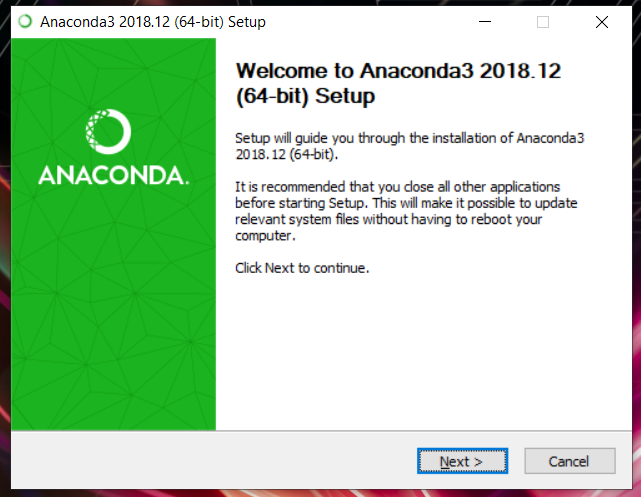
\includegraphics[width=3cm,height=3cm]{figures/1.png}
        \caption{gambar1}
        \label{awal}
        \end{figure}

    \item Lalu pada tampilan seperti gambar di bawah klik next.
    \begin{figure}[!htbp]
        \centering
        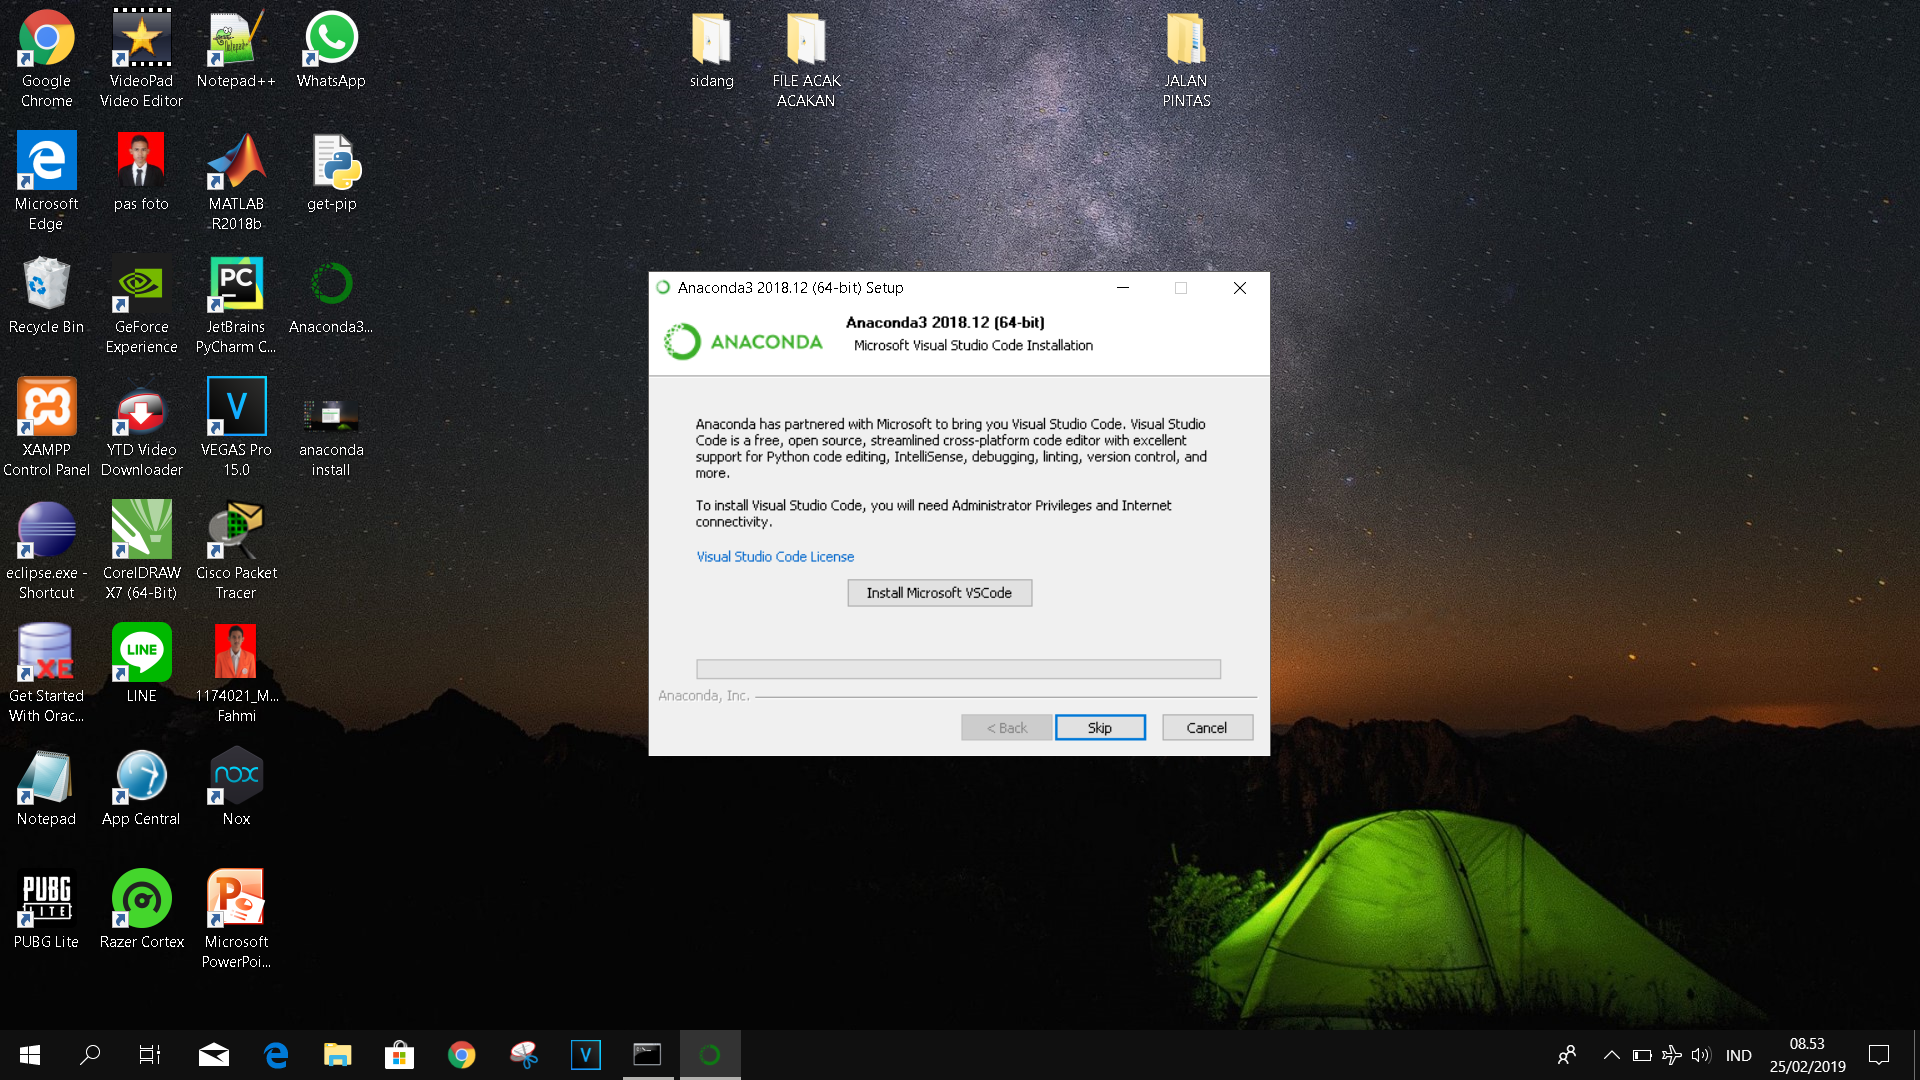
\includegraphics[width=3cm,height=3cm]{figures/2.png}
        \caption{gambar2}
        \label{next}
        \end{figure}

    \item Setelah itu setujui lisensi yang ada dengan mengklik I Agree
    \begin{figure}[!htbp]
        \centering
        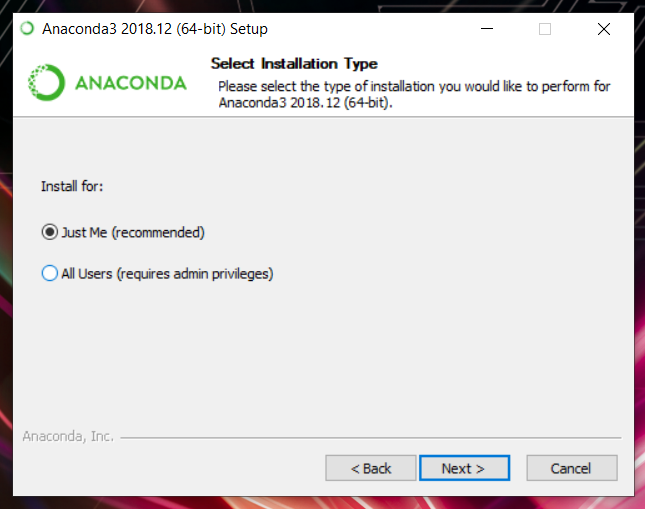
\includegraphics[width=3cm,height=3cm]{figures/3.png}
        \caption{gambar3}
        \label{lisensi}
        \end{figure}

    \item Tunggu instalasi selesai, lalu klik skip
    \begin{figure}[!htbp]
        \centering
        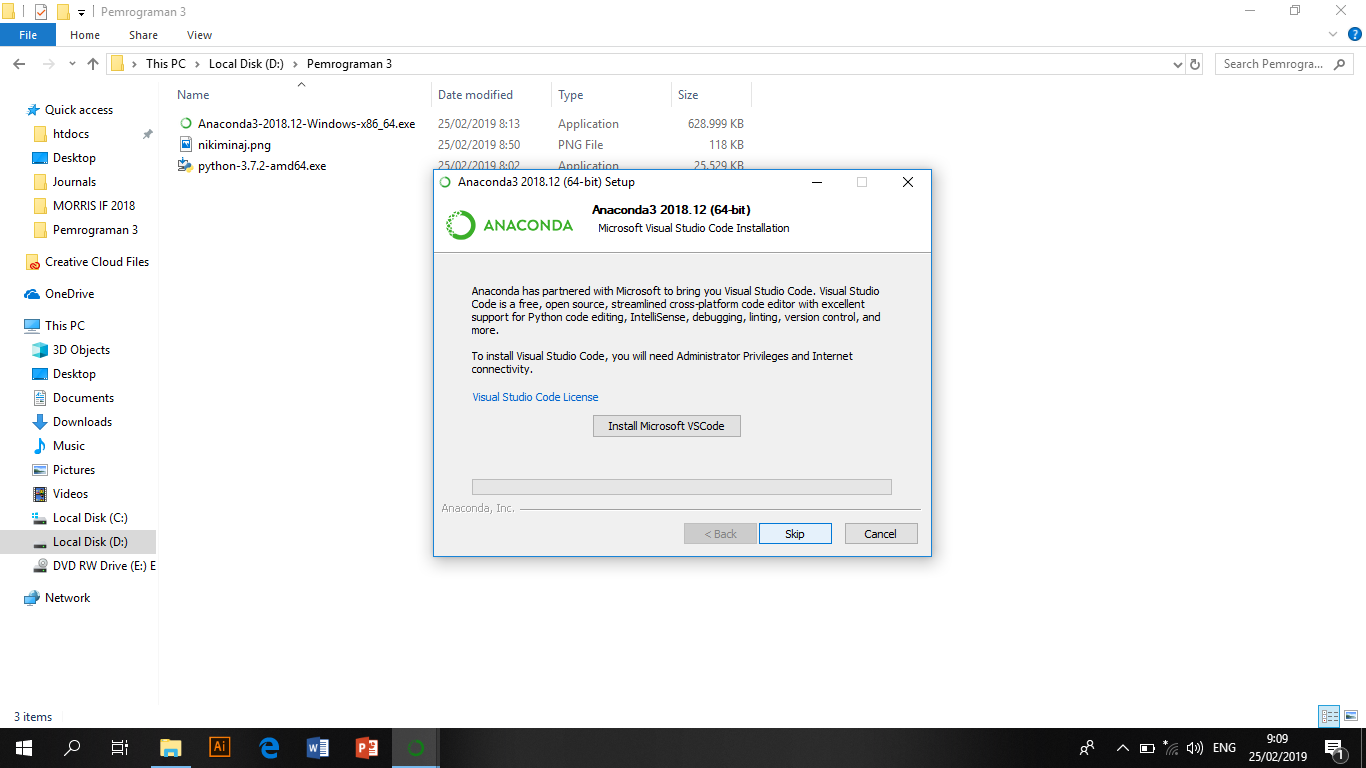
\includegraphics[width=3cm,height=3cm]{figures/4.png}
        \caption{gambar4}
        \label{skip}
        \end{figure}

    \item setelah itu klik finish, dan selesai yeay
    \begin{figure}[!htbp]
        \centering
        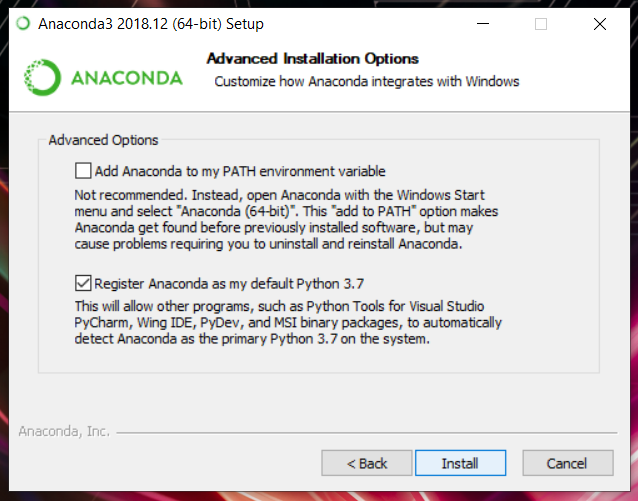
\includegraphics[width=3cm,height=3cm]{figures/5.png}
        \caption{gambar5}
        \label{selesai}
        \end{figure}
\end{enumerate}

\subsection{Menggunakan Spyder}
berikut adalah contoh dalam menggunakan spyder
\begin{figure}[!htbp]
    \centering
    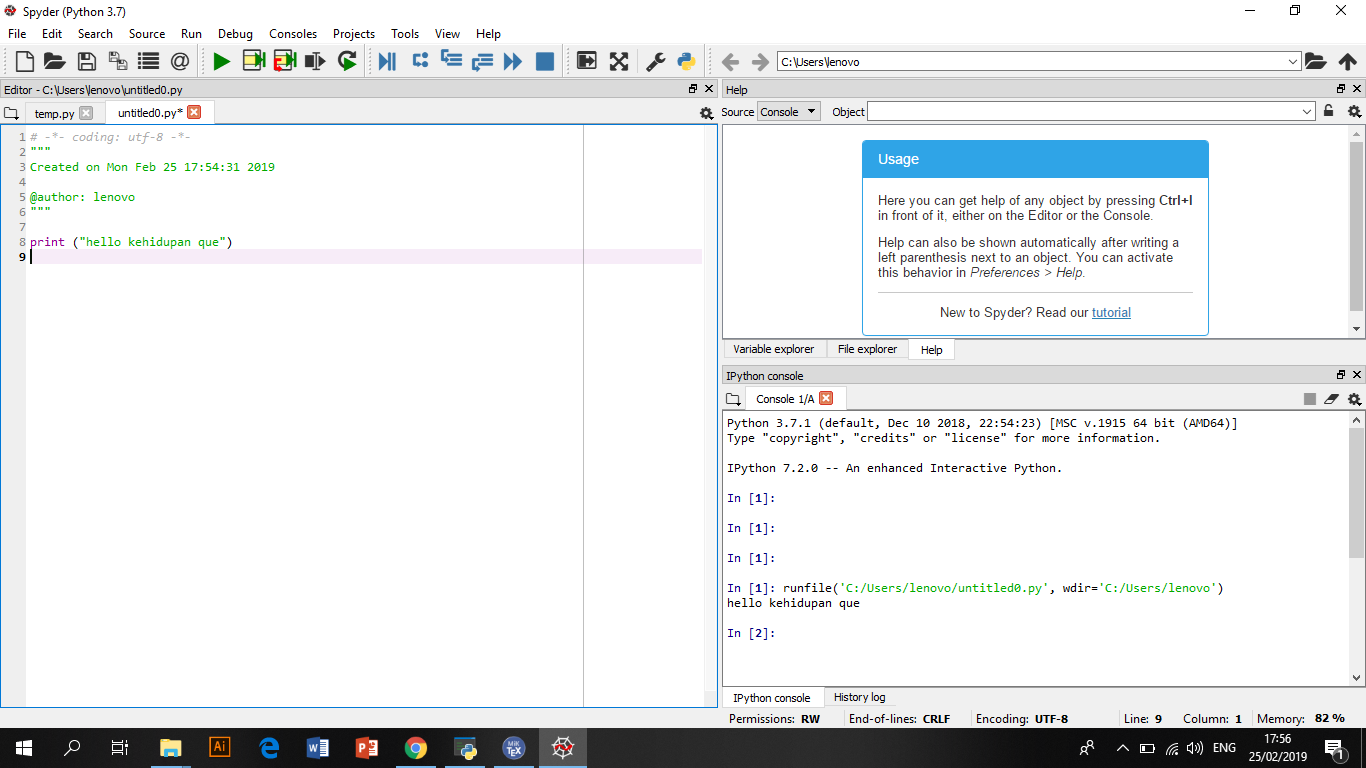
\includegraphics[width=3cm,height=3cm]{figures/6.png}
    \caption{gambar6}
    \label{spyder}
    \end{figure}
